\chapter{Conceptual Model}

Users will navigate to the application on an iPhone to begin using the system. Upon launching the app, a camera feed appears, as shown in Figure 5.1. They can press the camera icon to prompt the device to take a photo.

\begin{figure}[!h]
    \centering
    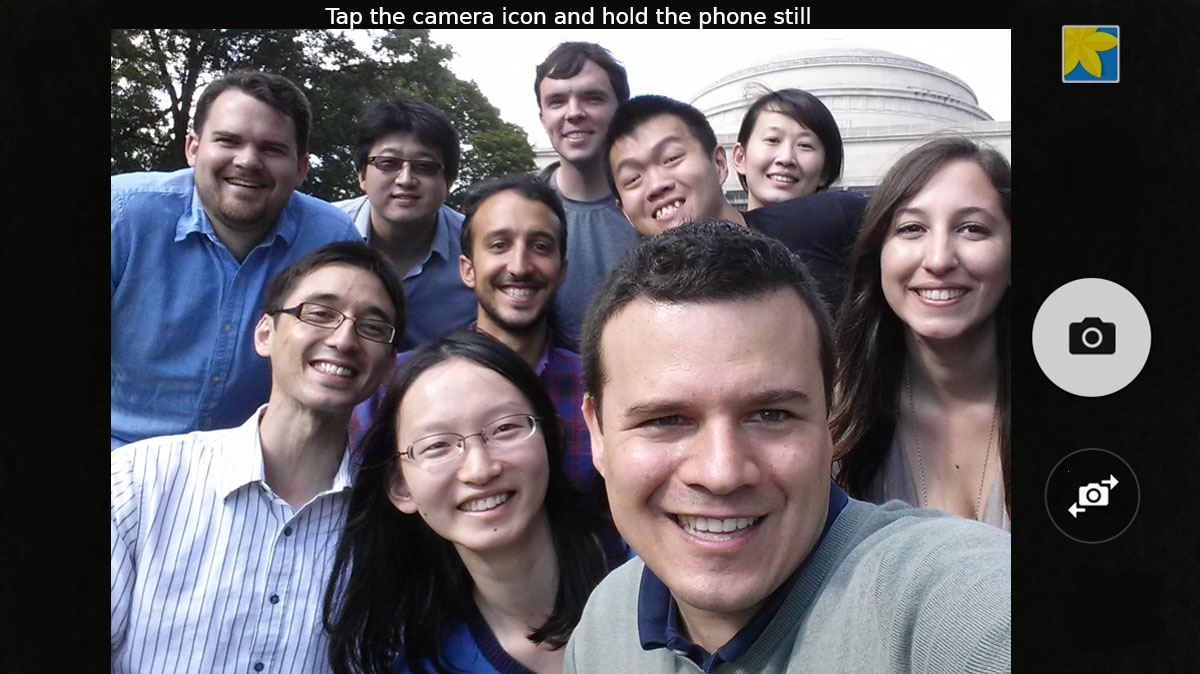
\includegraphics[width=0.75\textwidth]{conceptualmodel1}
    \caption{Mockup of camera user interface}
    \label{fig:conceptualmodel1}
\end{figure}

\pagebreak
After they has pressed the camera button, the application will wait until all subjects are in frame with their eyes open to capture the image. Upon capturing the image, they will be greeted with an alert asking whether they want to save the photo or reject it, as seen in Figure 5.2.

\begin{figure}[!h]
    \centering
    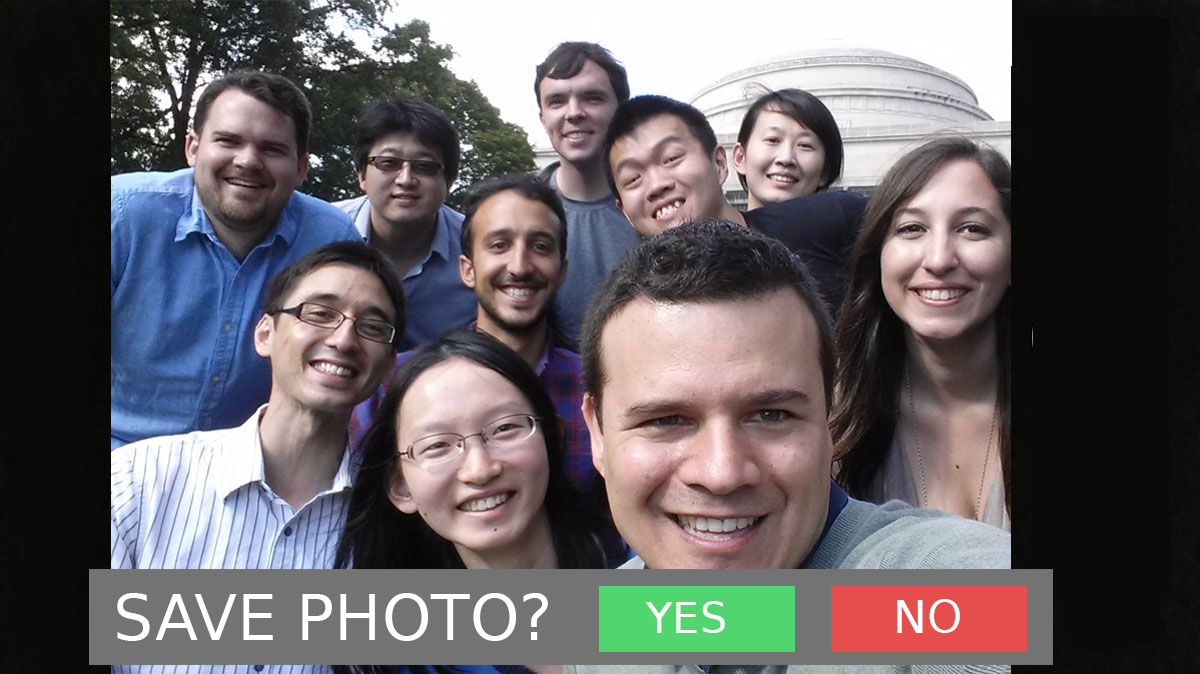
\includegraphics[width=0.75\textwidth]{conceptualmodel2}
    \caption{Mockup demonstrating the approval dialogue}
    \label{fig:conceptualmodel2}
\end{figure}

If the user chooses to accept the photo, then it will be saved to the user's storage and they will return to the camera screen. If the user chooses to discard the photo, then it will be delete and they will return to the camera.


